% This is samplepaper.tex, a sample chapter demonstrating the
% LLNCS macro package for Springer Computer Science proceedings;
% Version 2.20 of 2017/10/04
%
\documentclass{llncs}
%\documentclass[runningheads]{llncs}

%
\usepackage{graphicx}
\usepackage{epstopdf}
\usepackage[hyphens]{url}
\usepackage{hyperref}

% Used for displaying a sample figure. If possible, figure files should
% be included in EPS format.
%
% If you use the hyperref package, please uncomment the following line
% to display URLs in blue roman font according to Springer's eBook style:
% \renewcommand\UrlFont{\color{blue}\rmfamily}

\begin{document}
%
\title{IIT.SRC 2025 Evaluating Recommender Systems for Digital Library Datasets}
%
%\titlerunning{Abbreviated paper title}
% If the paper title is too long for the running head, you can set
% an abbreviated paper title here
%
\author{Ákos Lévárdy\thanks{Bachelor study programme in field: Informatics \\Supervisor: PaedDr. Pavol Baťalík, Faculty of Informatics and Information Technologies STU in Bratislava }}%\orcidID{0000-1111-2222-3333}}
%
%\authorrunning{F. Author et al.}
% First names are abbreviated in the running head.
% If there are more than two authors, 'et al.' is used.
%
\institute{Faculty of Informatics and Information Technologies STU in Bratislava \\
\email{\{abc,lncs\}@uni-heidelberg.de}}
%
\maketitle              % typeset the header of the contribution
%
\begin{abstract}
%With the increasing amount of digital content online, recommender systems play an important role in filtering out and helping users navigate large information spaces by generating personalized recommendations. Digital libraries can improve user experience by selecting the most effective and suitable recommendation systems. This study focuses on evaluating content-based recommender systems, which are specifically designed for digital library datasets. These content-based filtering methods analyze textual data from books to generate recommendations based on similarity between content features. The goal is to investigate different algorithms such as TF-IDF, LSA, GloVe or FastText, and testing them with different settings to assess their effectiveness in generating Top-N recommendations from book text data. 
%In order to fully evaluate these algorithms, we conduct experiments using multiple performance metrics like similarity, diversity, confidence or even coverage. Additionally, the performance of the algorithms is analyzed by tracking execution time and memory consumption. By benchmarking these factors, we provide information on the trade-offs between accuracy and computational efficiency for the different tested models. This research identifies the strengths and weaknesses of the selected algorithms for book recommendations, making it easier to navigate large digital collections.\\\\

As digital content continues to grow rapidly, users face increasing difficulty in finding relevant information efficiently—especially within large-scale digital libraries. Recommender systems help address this challenge by delivering personalized suggestions that improve user experience and reduce information overload. This study focuses on evaluating content-based recommender systems tailored for digital library datasets. These systems analyze textual data from books to generate recommendations based on similarities in content features. The goal is to compare algorithms such as TF-IDF, LSA, GloVe, and FastText under different settings, assessing their effectiveness in generating Top-N recommendations. To provide a comprehensive evaluation, the study uses multiple performance metrics including similarity, diversity, confidence, and coverage, while also measuring execution time and memory usage. By benchmarking these factors, we highlight the trade-offs between accuracy and computational efficiency, offering insights into the strengths and weaknesses of each algorithm for book recommendation tasks in digital libraries.
\keywords{Recommender System  \and  Content-Based  \and  Evaluation  \and  Performance Metrics  \and  Digital Library.}
\end{abstract}
%
%
%
\section{Introduction}
Making decisions in today’s digital world is not always easy. Whether choosing a product, a movie, or a travel destination, people are often faced with an overwhelming number of options and varying levels of information and trustworthiness. While some users know exactly what they are looking for and seek immediate answers, others are open to exploring new possibilities and expanding their knowledge \cite{Blanco201333}.

\textbf{Recommendation Systems (RS)} are designed to ease this process by predicting useful items, comparing them, and suggesting the most similar options based on user preferences. These systems have become essential tools for reducing information overload, especially with the rapid growth of big data \cite{Haruna2017}. By analyzing large volumes of textual data, they aim to understand users’ preferences and generate personalized recommendations \cite{Yan2024}.

The task of providing users with available options that match their needs and interests is increasingly important in today’s consumer society. Without a starting point—such as a list of relevant suggestions—users may feel overwhelmed or even choose to give up entirely. For example, trying to pick a movie from scratch without any recommendations can lead to decision fatigue. Recommender systems help prevent this by offering tailored suggestions that guide the user and reduce decision friction.

It’s also important to recognize the dual perspective from which recommendation systems operate \cite{Ricci20221}. On one hand, service providers aim to use these systems to sell more items, improve user satisfaction, or better understand customer behavior. On the other hand, from the user’s viewpoint, RS assist in discovering suitable items, recommending sequences, or even influencing others' decisions.

The core goal of RS is to personalize content and improve user experience by recommending books, movies, music, products, and more. For example, in a digital library which has loads of books available online, a recommender system might suggest books or even specific paragraphs based on a user’s reading history \cite{Zangerle2023}. These systems function by identifying relationships between users and the items they interact with—such as preferring historical documentaries over action films \cite{pub.1022525812}.

Various techniques are used to achieve this personalization. Collaborative filtering recommends items based on similar users’ preferences, while content-based filtering analyzes item features like genre or keywords. Hybrid approaches combine both for more accurate results \cite{Aymen2022896}. Regardless of the method, the aim is to help users discover relevant content they might not have found on their own.

That said, information systems must also account for the fact that user preferences can change over time. This phenomenon, known as concept drift, refers to unexpected changes in data patterns or behaviors that can significantly affect the system’s prediction accuracy \cite{Sun2024}. Recommender systems need to be adaptive in order to stay effective over long periods.

Recommendation systems differ from search engines, although both are used to navigate large amounts of information. While search engines retrieve content based on keywords, recommender systems make predictions based on user behavior and inferred interests \cite{De_Nart201484}.

This paper focuses on evaluating and comparing different recommendation algorithms for suggesting books and their parts based on textual content. Algorithms such as TF-IDF, LSA, and BERT will be tested to assess how effectively they generate recommendations. Evaluation will consider metrics like similarity, diversity, confidence, and coverage \cite{Gunawardana2022547}, along with performance factors such as execution time or memory usage.

%The goal is to strike a balance between accuracy and efficiency, ultimately creating a system that helps users explore large digital libraries more effectively and enjoyably.

%As the internet and technology continue to evolve rapidly, the amount of information available online has grown significantly, covering areas like online shopping, government services, entertainment, education, and much more. With so much information out there, it’s easy for users to feel overwhelmed. This is where Recommender Systems (RS) come in. These systems are essential for improving the user experience by helping people find the most relevant information, saving time and effort. Rather than showing everything available, they predict what a user is most likely to be interested in, offering suggestions based on their needs and preferences. Recommender systems are powerful tools that make it easier for users to find content that suits their tastes, whether it’s a book, movie, product, or music.\\
%%
%The main idea behind recommender systems is to personalize the content shown to each user \cite{Aymen2022896}. By using algorithms that analyze past behavior and preferences, these systems suggest items that align with a person’s individual interests. For example, in a digital library, a recommender system suggests books that might be of interest based on the user’s reading history. \\
%The design of these systems varies depending on the type of content being recommended, whether it’s movies, books, or any other type of media. A movie recommendation system would work differently from a book recommender system because of the specific characteristics \cite{pub.1036183961}.\\
%%
%There are different methods that recommender systems use to predict what a user might like. Collaborative filtering looks at the behavior of similar users and suggests items based on what others with similar tastes have liked. Content-based filtering, on the other hand, analyzes the features of the items themselves, such as genre, author, or keywords, and recommends similar items based on what the user has liked before. Some systems even use a mix of both approaches, known as Hybrid methods, to make better and more accurate suggestions. Regardless of the method, the main goal is to help users find content that is most relevant to them by understanding the connections between what they like and what’s available.\\
%%
%At the core of these systems is the idea that there are relationships between what users are interested in and the items they interact with. For instance, if a user watches a historical documentary, they are more likely to enjoy another documentary on a similar topic, like ancient history, than a completely different genre, like action movies \cite{pub.1022525812}. Recommender systems aim to identify these relationships and help users discover content they might not have come across on their own.\\
%%
%The focus of this paper was on evaluating different algorithms and comparing their performance and results. This evaluating system is specifically set for recommending books and parts or paragraphs of these books based on their textual content. With the vast number of books available, it’s important to have an efficient system that can help users find books they will enjoy \cite{Zangerle2023}. The system will test different algorithms, including TF-IDF, LSA, BERT and so on which are all designed to analyze text and make recommendations. Each of these algorithms works differently, so it’s important to compare them and see how well they perform in recommending books and paragraphs.\\
%%
%To evaluate the effectiveness of these algorithms, the system will be tested based on several factors, like similarity, diversity, confidence and coverage \cite{Gunawardana2022547}. These metrics help measure how well the system recommends books that match the user’s interests, how varied the suggestions are, and how much of the available content is covered. Additionally, the project will also look at how efficient the system is by monitoring execution time, memory usage, and CPU performance. This allows us to balance both accuracy and efficiency, ensuring the system works well without overloading the computer. \\
%By testing these algorithms and considering both their effectiveness and efficiency, this project aims to provide a useful tool for digital libraries, helping users find the right books while improving their overall experience. Ultimately, the goal is to make the book discovery process easier and more enjoyable, so users can explore large collections without feeling lost.\\









%\subsection{A Subsection Sample}
%Please note that the first paragraph of a section or subsection is
%not indented. The first paragraph that follows a table, figure,
%equation etc. does not need an indent, either.

%Subsequent paragraphs, however, are indented.

%\subsubsection{Sample Heading (Third Level)} Only two levels of
%headings should be numbered. Lower level headings remain unnumbered;
%they are formatted as run-in headings.

%\paragraph{Sample Heading (Fourth Level)}
%The contribution should contain no more than four levels of
%headings. Table~\ref{tab1} gives a summary of all heading levels.







%\subsubsection{Understanding Recommendation Systems}
%Making decisions is not always easy. People are frequently presented with an overwhelming number of options when picking a product, a movie, or a destination to travel to, and each option comes with different levels of information and trustworthiness. \\
%While there are many situations in which users know exactly what they are looking for and would like immediate answers, in other cases they are willing to explore and extend their knowledge \cite{Blanco201333}.\\\\
%The main purpose of \textbf{Recommendation Systems} is to predict useful items, select some of them and after comparing them, the system recommends the most accurate ones.\\ 
%These Personalized recommendation systems are emerging as appropriate tools to aid and speed up the process of information seeking, considering the dramatic increase in big data \cite{Haruna2017}. They need to handle a large amount of textual data in order to accurately understand users’ reading preferences and generate corresponding recommendations \cite{Yan2024}. \\
%%
%Because of this number of detail from all of the items, recommendation systems are becoming increasingly important. They help reduce options and offer better suggestions for the user so that they will have a personalized list to select their favourite. Fast and efficient access to information is essential in any field of study. \\\\
%%
%%Similarly, \textbf{Search Engines} are essential for navigating the vast amount of information available online. They make it possible for people to quickly look up solutions, learn new things, and browse the wide variety of resources on the internet. Search engine optimization is now necessary to guarantee that search engines deliver relevant results, quick search times, and a top-notch user experience given the explosive growth of online information.\\
%%A search engine is essentially a software that finds the information the user needs using keywords or phrases. It delivers results rapidly, even with millions of websites available online.
%%The importance of speed in online searches is highlighted by how even minor delays in retrieval can negatively affect users' perception of result quality \cite{pub.1171882357}.\\
%%
%While both Recommendation Systems (Information Filtering techniques) and Search Engines (Information Retrieval techniques) aim to help users navigate all this information, they do it differently. Personalized recommendation systems make suggestions based on past user behavior and preferences, whereas search engines use keyword-based searches to retrieve content from a selection of sources \cite{De_Nart201484}.\\








%
%Information systems often deal with changing data over time. The term called Concept drift describes when sometimes the patterns or behaviors in the data change unexpectedly which affects how the system makes predictions \cite{Sun2024}.\\
%It is also crucial to distinguish on whose behalf the role of the recommendation system is played. One role could be the service providers role, who would like to sell more items, increase user satisfaction or better understand what the user wants with recommendations \cite{Ricci20221}. The other role is from the users point of view the recommendation system can be helpful with tasks such as finding some good items, recommending a sequence or influencing others to consider particular products.\\
%The task to provide users with currently available options for products that fit their requirements and interests is very important in todays consumer society. These products are mostly supplied by inputs \cite{Philip2014} , sometimes even matching the users distinct tastes.\\
%%
%When someone is trying to find a movie to watch, it would be hard for them to start searching without any starting options. After all a blank page and no suggestions to choose from might even make the user decide not to pick anything.

Recommending items can be done in a variety of ways. Several types of recommendation systems exist, and their methods of operation differ \cite{Roy2022}. Here are the different recommendation system types:\\\\
%
%
%\textbf{Content-Based Filtering} works in a way that it creates user profiles and suggests the individual items or products based on the users past choices with similar items. The items have various features and characteristics which connect them.\\
\textbf{Content-Based Filtering} recommends items based on a user's previous choices or interactions by finding similarities between the items the user has shown interest in and other items with similar features (e.g., genre, attributes, keywords) \cite{pub.1034486657}.\\
This approach focuses primarily on the item's characteristics rather than relying on other users' preferences.\\
\textbf{Collaborative Filtering} relies more on preferences of other users and their behaviour. The point is that users who had similar interests before will have them again in the future for new items. This technique relies on having user related data, feedback that could be either explicit (ratings) or implicit (passive user behaviour).
\begin{figure}
\centering
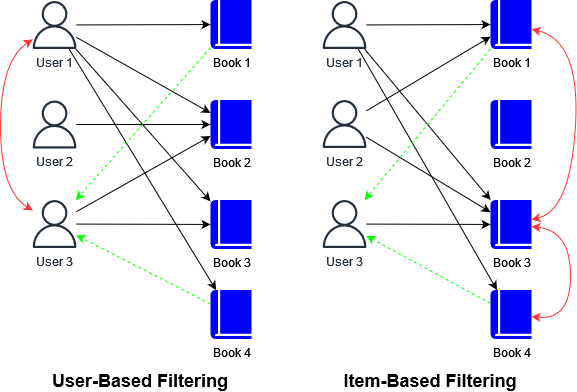
\includegraphics[width=0.8\textwidth]{img/collaborative_example.png}
%
\includegraphics[width=\textwidth]{fig1.eps}
\caption{Illustration of Memory-based CF recommendation.} \label{fig:collaborative_example}
\end{figure}\\
\textbf{Context-Aware} recommendation systems are adding contextual factors to the rating process, where the recommended item is based on the users explicit ratings, the items implicitly inferred ratings and also the contextual variables. The variables for example when recommending a movie can be the location from where the user watches the movie, the time and the companion who the user watches the movie with.\\
\textbf{Popularity-Based} recommendations offer products that are popular or well-liked by a lot of users. They assume that these popular items are likely to be of interest to the majority of users, not considering their personal preferences.\\
\textbf{Demographic} recommendation systems are recommending items based on a demographic profile of the user. They categorize the users from their personal attributes and try to make user stereotypes.\\
\textbf{Knowledge-Graphs} use a network of data where items are linked through their features. Showing how items relate to one another and connecting them with more information \cite{Imene2022488}.
\begin{figure}
\centering
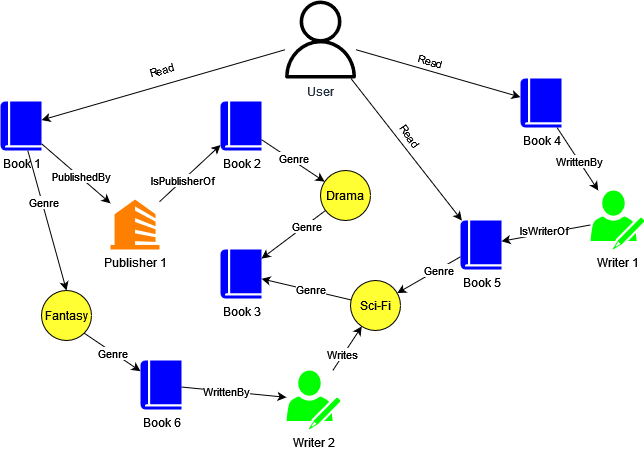
\includegraphics[width=0.8\textwidth]{img/knowledge_graph_example.png}
%
\includegraphics[width=\textwidth]{fig1.eps}
\caption{Illustration of KG-aware recommendation.} \label{fig:knowledge_graph_example}
\end{figure}\\
\textbf{Utility-Based} systems generate the recommendations by computing the utility of each item for the user. The utility of an item refers to how valuable it is to a user and is calculated using a utility function which combines different factors of the user's preferences \cite{Burke2002331}.\\
\textbf{Deep Learning-Based} are trying to find complex patterns in the users behaviour and the items features using deep learning algorithms and neural networks. These models can locate hidden links and can offer highly customized recommendations.\\
\textbf{Hybrid methods} try to combine the useful characteristics of both collaborative filtering and content-based filtering methods. They take into account both the users past preferences and the preferences of other people who might share the users taste \cite{melville:aaai02}. \\\\
%
The most popular techniques used are the Collaborative Filtering, Content-Based Filtering and the Hybrid method \cite{pub.1072601078}. This paper will focus on comparing different algortihms that are used for Content-Based Filtering, since trying to recommend books and their paragraphs in digital libraries relies on the textual content of them.


\section{System Decription}
%\textbf{SYSTEM DESCRIPTION}\\
\textbf{Extracting Information and Building a Dataset}\\
First, the books, meaning their whole text and summaries were extracted from the digital library and separeted into JSON files, each file contained one books whole data, which was even more separated into sentences, pages and paragraphs.\\
From extracting metadata of the books from the digital library, the dataset had 403 different books short summaries that were used in the testing phase. On the other hand, the full text extraction resulted in a dataset of 45 163 paragraphs where the average paragraph word count was around 63.73 words and the longest paragraph had 2016 words.\\
% the algorithms were tested with the paragraphs of the books\\
%Each algorithm embedded or vectorized all of the paragraphs as they required and got an input paragraph that they also embedded or vectorized, computed cosine similarity between the input and each other paragraph in the datased, based on mostly cosine similarity they were sorted and top 5 paragraphs were returned as the algorithms recommendations.\\\\
Each algorithm began by embedding or vectorizing all of the paragraphs in the dataset according to its specific requirements. This process involved transforming the text into numerical representations, such as vectors, which could then be compared based on their similarities. After the entire dataset of paragraphs was embedded or vectorized, the system received an input paragraph. This input paragraph was also embedded or vectorized in the same manner as the rest of the dataset. Once the input paragraph was transformed, the system calculated the cosine similarity between the input paragraph’s vector and the vectors of each of the other paragraphs in the dataset.\\\\
The cosine similarity measure was used to determine how closely related the input paragraph was to each of the other paragraphs. Cosine similarity is a mathematical measure that assesses the angle between two vectors, with a smaller angle indicating higher similarity. Based on the computed cosine similarity scores, the paragraphs in the dataset were sorted, with the most similar ones ranked at the top. From this sorted list, the top 5 most similar paragraphs were selected as the algorithm's recommendations for the input paragraph. These top 5 paragraphs were returned to the user as the most relevant or similar ones based on the cosine similarity metric.\\\\
%
%
\textbf{Descriptions of the Algorithms Used}\\
In the context of academic book recommendations, a variety of content-based algorithms can be used to extract meaningful patterns and relationships from textual data. These algorithms differ in their approach to representing and analyzing documents, words and textual data. Below is an overview of common algorithms, highlighting their methodology and key characteristics:\\\\
\textbf{TF-IDF (Term Frequency - Inverse Document Frequency)} creates two matrices that are interrelated, trying to figure out the relevancy of a given term (word) to a document given a larger body of documents.\\\\
TF means how often a given word occurs in the given document, because words that occur frequently are probably more important. DF means how often the given word occurs in an entire set of documents, but this does not have to mean the word is important, it just shows common words that appear everywhere. So using Inverse DF shows how often the word appears in a document, over how often it appears everywhere.\\\\
\textbf{BoW (Bag of Words)} creates a set of vectors containing the count of word occurrences in the document. Unlike TF-IDF, BoW just counts the occurrences of unique words and puts them in its vocabulary so each word becomes a feature or dimension. Each document is represented as a vector based on the frequency of words from the vocabulary. The term-document matrix represents the documents as rows and the unique words as columns with cells showing frequency.\\\\
\textbf{GloVe (Global Vectors for Word Representation)} is a word embedding model that builds a co-occurrence matrix where rows represent the words, columns represent the context words and each cell contains the frequency with which the word and context word co-occur within a specified window. The matrix is factorized to learn word embeddings. After training GloVe produces embeddings for all words in the vocabulary.\\\\
\textbf{LSA (Latent Semantic Analysis)} is a model for extracting and representing the contextual-usage meaning of words by statistical computations applied to a large corpus of documents. It uses Singular Value Decomposition (SVD) and Rank lowering (Dimensionality reduction). The SVD splits the Matrix of document by keyword into three matrices, which are topic by keyword, document by topic and the diagonal matrix.\\\\
\textbf{FastText} breaks words into character n-grams and learns embeddings for these subwords. It can handle words that are out of the vocabulary, because it models character n-grams and not words. For output it produces dense, fixed-length word vectors that have the additional subword information.\\



\begin{table}
\caption{Results of Different Algorithms - Using Paragraphs}\label{tab1}
\centering
\begin{tabular}{|l|l|l|l|l|}
\hline
\textbf{Algorithm} & \textbf{Avg Similarity} & \textbf{Avg Confidence} & \textbf{Avg Diversity} &  \textbf{Avg Elapsed\_time (s)} \\ 
\hline
TF-IDF      & 0.41  & 0.04  & 0.59  & 13.86  \\ \hline
BoW         & 0.50  & 0.13  & 0.50  & 13.25  \\ \hline
FastText    & 0.98  & 0.00  & 0.02  & 42.81 \\ \hline
GloVe       & 0.99  & 0.00  & 0.01  & 14.39 \\ \hline
LSA         & 0.66  & 0.02  & 0.34  & 12.66   \\ \hline

\end{tabular}
\end{table}

\begin{table}
\caption{Results of Different Algorithms - Using Summaries}\label{tab2}
\centering
\begin{tabular}{|l|l|l|l|l|}
\hline

\textbf{Algorithm} & \textbf{Avg Similarity} & \textbf{Avg Confidence} & \textbf{Avg Diversity} & \textbf{Avg Coverage (\%)} \\ 
\hline
TF-IDF    & 0.18                    & 0.092               & 0.82                & 3.28 \\ \hline
BoW                 & 0.256                   & 0.108               & 0.744               & 4.14 \\ \hline
FastText            & 0.993                   & 0.005               & 0.007               & 37.44 \\ \hline
GloVe               & 0.983                   & 0.021               & 0.017               & 8.14 \\ \hline
LSA                 & 0.497                   & 0.133               & 0.503               & 4.17 \\ \hline

%Word2Vec            & 1.0                     & 0.0                 & 0.0                 & 56.6 \\ \hline
%Doc2Vec             & 1.0                     & 0.001               & 0.0                 & 77.44 \\ \hline
%BERT                & 0.445                   & 0.119               & 0.555               & 7.02 \\ \hline
%BM25                & 0.836                   & 0.188               & 0.164               & 6.63 \\ \hline
%LDA                 & 0.991                   & 0.029               & 0.009               & 14.96 \\ \hline

\end{tabular}

\end{table}


\section{Experimental Results}
%\noindent
%\textbf{EXPERIMENTAL RESULTS}\\\\
% SHOW EXAMPLES OF VECTORS OR WIEGHTS THAT ALGOS USE\\\\
% CPU / MEMORY usage graphs\\\\
%
The experiment results from the two tables present the performance of different algorithms evaluated based on two distinct content types: paragraphs and summaries. The metrics used to evaluate the algorithms include average similarity, confidence, diversity, and coverage. Here's a brief description of these metrics:
\textbf{Average similarity} indicates how closely the recommendations align with the input content, with higher values representing more relevant recommendations. \textbf{Confidence} measures the algorithm’s certainty about the relevance of its recommendations. Higher values suggest the algorithm is more confident in its suggestions. \textbf{Diversity} reflects the variety of recommendations made. A higher diversity value indicates that the algorithm provides a broader range of suggestions.
\textbf{Coverage} refers to the percentage of items from the dataset that the algorithm is able to recommend. A higher coverage indicates that the algorithm suggests a larger portion of the available items.

\noindent
\textbf{Performance on Paragraphs} is shown in the first table, which contain more detailed information compared to summaries. As such, the metrics for paragraphs may show higher values for relevance and coverage, since longer text provides more context.

\noindent
\textbf{FastText} stands out with the highest \textbf{average similarity} of 0.98, meaning its recommendations are highly relevant. However, this comes at the cost of \textbf{average elapsed time} (42.81 seconds), indicating that it is slower compared to other algorithms. It performs well in terms of relevance but is slower in processing. \textbf{TF-IDF} and \textbf{BoW}, while being faster (13.25 and 13.86 seconds for \textbf{avg\_elapsed\_time}), show lower \textbf{average similarity} (0.41 and 0.50, respectively), meaning their recommendations are less aligned with the user’s preferences. These algorithms are quicker but less accurate. \textbf{GloVe} and \textbf{LSA} perform moderately well in terms of similarity, with \textbf{LSA} being slightly faster than \textbf{GloVe}.\\
Overall, the first table highlights the trade-off between accuracy and efficiency: algorithms like \textbf{FastText} provide more accurate results but take more time to process, while others like \textbf{TF-IDF} and \textbf{BoW} are quicker but less precise in their recommendations.

\noindent
\textbf{Performance on Summaries} is shown in the second table. Since summaries are shorter and less detailed than paragraphs, the results show lower accuracy (i.e., \textbf{average similarity}) but provide a broader view of how the algorithms behave with concise content. The coverage of each algorithm was set to return recommended items above the same dynamically set threshold.\\
\noindent
\textbf{FastText} again performs the best in \textbf{average similarity} with a value of 0.993, which indicates its ability to generate highly relevant recommendations. It also has the highest \textbf{coverage} at 37.44\%, suggesting it can recommend a large portion of the dataset. However, its \textbf{confidence} and \textbf{diversity} values are lower, suggesting that while the recommendations are relevant, they may be more focused and less diverse. 
\noindent
\textbf{GloVe} performs well with an \textbf{average similarity} of 0.983, meaning its recommendations are quite relevant, though its \textbf{coverage} is only 8.14\%, implying it covers fewer items from the dataset compared to algorithms like \textbf{FastText}.
\noindent
\textbf{LSA} shows a moderate \textbf{average similarity} of 0.497, indicating that its recommendations are less aligned with the summaries compared to \textbf{FastText} and \textbf{GloVe}. However, it strikes a good balance between \textbf{diversity} (0.503) and \textbf{coverage} (4.17\%), suggesting that \textbf{LSA} provides more varied recommendations but with less precision in terms of relevance.
\noindent
\textbf{TF-IDF} has the lowest \textbf{average similarity} value of 0.18, indicating that its recommendations are not closely aligned with the user's preferences. However, it performs well in terms of \textbf{diversity} (0.82), suggesting that it provides a variety of recommendations, although these are less relevant. Its \textbf{coverage} is low at 3.28\%, meaning it can only recommend a small portion of the available dataset.
\noindent
Overall, the table illustrates the trade-off between relevance, diversity, and coverage. Algorithms like \textbf{FastText} and \textbf{GloVe} provide more relevant recommendations but vary in their coverage of the dataset. \textbf{TF-IDF} provides more diversity but less relevance, while \textbf{LSA} offers a balance between diversity and coverage at the expense of similarity. These metrics allow us to assess the strengths and weaknesses of each algorithm in terms of their ability to meet the requirements of a recommendation system.\\


\section{Future Work}
%\noindent
%\textbf{FUTURE WORK}\\
Future work could explore improving the efficiency of the algorithms by implementing more advanced optimization techniques to reduce the computational time and memory usage, especially for models like FastText. Additionally, hybrid approaches combining content-based filtering with collaborative filtering could be tested to enhance the accuracy of recommendations by considering both item features and user preferences. Further evaluation of these algorithms could involve larger datasets and more diverse types of content to assess the scalability and generalization of the models. Exploring deep learning-based methods, such as using transformer models or neural networks, could also be an interesting direction for improving recommendation quality. Finally, incorporating user feedback to dynamically adjust recommendations in real-time could be an important area of focus.\\\\
%
\section{Conclusions}
%\textbf{CONCLUSIONS}\\
This study focused on evaluating content-based recommender systems for digital library datasets, comparing several algorithms such as TF-IDF, LSA, FastText, GloVe, and BoW. The goal was to assess how well these algorithms can generate recommendations based on the textual content of books and their paragraphs, and how efficiently they perform under different computational loads.\\
From the results of the performance metrics, it is evident that there are trade-offs between relevance, diversity, and efficiency. Algorithms like FastText and GloVe offer highly relevant recommendations but tend to require more computational resources in terms of processing time. On the other hand, methods such as TF-IDF and BoW are faster but offer lower similarity, meaning the recommendations are less aligned with the user’s preferences. LSA provides a balance between similarity and diversity, though it still lags behind the best-performing models in terms of relevance.\\\\
Additionally, the analysis of coverage showed how well the algorithms could recommend a wide range of items from the dataset. FastText, while highly relevant, exhibited lower diversity and coverage compared to GloVe, indicating that its recommendations are more focused. In contrast, TF-IDF offered higher diversity but lower relevance, meaning it could recommend a wider variety of items.\\
The findings suggest that hybrid models combining content-based filtering with collaborative filtering techniques could improve recommendation quality, as they would leverage both textual content and user behavior data. Further research could explore deep learning models, such as neural networks, to detect more complex patterns in large datasets and improve recommendations.\\
In conclusion, this research provides valuable insights into the strengths and weaknesses of various content-based algorithms for digital libraries, offering a framework to optimize recommendation systems. \\\\






%\begin{table}
%\caption{Table captions should be placed above the
%tables.}\label{tab1}
%\begin{tabular}{|l|l|l|}
%\hline
%Heading level &  Example & Font size and style\\
%\hline
%Title (centered) &  {\Large\bfseries Lecture Notes} & 14 point, bold\\
%1st-level heading &  {\large\bfseries 1 Introduction} & 12 point, bold\\
%2nd-level heading & {\bfseries 2.1 Printing Area} & 10 point, bold\\
%3rd-level heading & {\bfseries Run-in Heading in Bold.} Text follows & 10 point, bold\\
%4th-level heading & {\itshape Lowest Level Heading.} Text follows & 10 point, italic\\
%\hline
%\end{tabular}
%\end{table}


%\noindent Displayed equations are centered and set on a separate
%line.
%\begin{equation}
%x + y = z
%\end{equation}
%Please try to avoid rasterized images for line-art diagrams and
%schemas. Whenever possible, use vector graphics instead (see
%Fig.~\ref{fig1}).

%\begin{figure}
%
\includegraphics[width=\textwidth]{fig1-eps-converted-to.pdf}
%\caption{A figure caption is always placed below the illustration.
%Please note that short captions are centered, while long ones are
%justified by the macro package automatically.} \label{fig1}
%\end{figure}

%\begin{theorem}
%This is a sample theorem. The run-in heading is set in bold, while
%the following text appears in italics. Definitions, lemmas,
%propositions, and corollaries are styled the same way.
%\end{theorem}
%
% the environments 'definition', 'lemma', 'proposition', 'corollary',
% 'remark', and 'example' are defined in the LLNCS documentclass as well.
%
%\begin{proof}
%Proofs, examples, and remarks have the initial word in italics,
%while the following text appears in normal font.
%\end{proof}
%For citations of references, we prefer the use of square brackets
%and consecutive numbers. Citations using labels or the author/year
%convention are also acceptable. The following bibliography provides
%a sample reference list with entries for journal
%articles~\cite{ref_article1}, an LNCS chapter~\cite{ref_lncs1}, a
%book~\cite{ref_book1}, proceedings without editors~\cite{ref_proc1},
%and a homepage~\cite{ref_url1}. Multiple citations are grouped
%\cite{ref_article1,ref_lncs1,ref_book1},
%\cite{ref_article1,ref_book1,ref_proc1,ref_url1}.
%
% ---- Bibliography ----
%
% BibTeX users should specify bibliography style 'splncs04'.
% References will then be sorted and formatted in the correct style.
%

%
%\begin{thebibliography}{8}
%\bibitem{ref_article1}
%Author, F.: Article title. Journal \textbf{2}(5), 99--110 (2016)
%
%\bibitem{ref_lncs1}
%Author, F., Author, S.: Title of a proceedings paper. In: Editor,
%F., Editor, S. (eds.) CONFERENCE 2016, LNCS, vol. 9999, pp. 1--13.
%Springer, Heidelberg (2016). \doi{10.10007/1234567890}
%
%\bibitem{ref_book1}
%Author, F., Author, S., Author, T.: Book title. 2nd edn. Publisher,
%Location (1999)
%
%\bibitem{ref_proc1}
%Author, A.-B.: Contribution title. In: 9th International Proceedings
%on Proceedings, pp. 1--2. Publisher, Location (2010)
%
%\bibitem{ref_url1}
%LNCS Homepage, \url{http://www.springer.com/lncs}. Last accessed 4
%Oct 2017
%\end{thebibliography}
 
 
 
 
 \bibliographystyle{splncs04}
 \bibliography{literature}
 
 
\end{document}
